%*****************************************
\chapter{ \textbf{Theoretical framework} }\label{ch:Theoretical}
%*****************************************
\vspace{0.5cm} 
%============================================================================================================================================================

\section{Introduction}\label{sec:Intro}

During the last years, the exoplanetary astrophysics field has become stronger and stronger. Searching for new worlds revolving around other stars has imposed important challenges in current science such as planetary formation models, observational and instrumentation challenges, for example. With the arrival of new instruments, each time more powerful, Astronomers are able to study and characterize these distant worlds to lately compare them with our solar system. In spite of it, we still have a long way to go in studying and understanding these interesting objects.\\

This project is mainly focused on studying exoplanets with rings, orbiting around young stars. At the moment, there is a lot of debate on whether or not, we have observed some features in light curves which could be explained by transiting exoplanetary rings in front of a parent star. On top of that, it is well-known that rings are not an exception in our solar system, where we can observe majestic structures as Saturn's rings or modest ones as the other gaseous-planets or even asteroids as Chariklo. As there is no clear consensus at what time exactly during the stellar life and planetary formation, rings could be formed, we aimed to enhance our chance of detecting these structures while studying young stars based on the occurrence rate and detection probability studied in \autoref{ch: Model}. This particular stellar population is expected to be forming planets at early stages which makes them good candidates in our search. The targeted field of study is known as Sco OB2 or ScoCen, a really young OB stellar stellar association lying at a distance of $\sim100-150 \textnormal{pc}$ from the Sun. ScoCen is the closest OB association that has recently formed stars and it is located between the constellations of Scorpius, Centaurus, Lupus, and Crux in the southern hemisphere.\\ 

In addition, all the characterization of astrophysical sources is mainly dependent on the distance relative to the observer. Therefore, aiming for excellent measurements of distance is essential to properly address our study. A few years ago in $2013$, the \textit{Gaia} mission was launched to measure with high precision the parallaxes and proper motions of stars in the Milky Way galaxy. \textit{Gaia} samples the whole celestial sphere, and provides extremely accurate measurements for the ScoCen OB association, allowing us to study in detail a larger number of stars as never before.\\  

In this chapter, a brief introduction to planet-formation and exoplanetary rings is provided. Also, we describe the most relevant features of the \textit{Gaia} mission and a general description of the ScoCen OB association. 
%==============================================================================================================================
\section{The Gaia mission}\label{sec:Gaiamission}

Astrometry is the astronomical discipline concerned with the accurate measurement and study of the (changing) positions of celestial objects. The number of stars for which ground-parallaxes were available until mid-1990's was limited just to a small sample over $8\,000$ \cauthor{1995gcts.book.....V} (\citeyear{1995gcts.book.....V}). The situation changed dramatically in $1997$ with the \textit{Hipparcos} satellite of the European Space Agency (\textit{ESA}), which measured the absolute parallax with a milli-arcsecond accuracy of as many as $117\,995$ objects (ESA $1997$). On 19th December 2013 \textit{Gaia} was launched and arrived at its operating point, the Lagrange point of the Sun-Earth-Moon system, a few weeks later (\cauthor{2016A&A...595A...1G} \citeyear{2016A&A...595A...1G}). Unlike its predecessor mission \textit{Hipparcos}, which selected its targets for observation based on a predefined input catalog loaded on board  \cauthor{1993BICDS..43....5T} (\citeyear{1993BICDS..43....5T}), \textit{Gaia} performs an unbiased, flux-limited survey of the sky. This difference was primarily motivated by the fact that an all-sky input catalog at the spatial resolution of \textit{Gaia} that is complete down to $20$th mag, does not exist (\cauthor{2016A&A...595A...1G} \citeyear{2016A&A...595A...1G}). On the other hand, and interesting and remarkable point is that the \textit{Gaia} collaboration does not have data rights. Thus, after processing, calibration, and validation inside the DPAC, data are made available to the world without limitations; this also applies to the photometric and solar system object science alerts (\cauthor{2016A&A...595A...1G} \citeyear{2016A&A...595A...1G}).\\ %Back in the days, the \textit{Gaia} mission was planned to be originally as a Global Astrometric Interferometer for Astrophysics called \textit{GAIA}, but the final design changed, so did the spelling.\\

The scientific aim of the design reference \textit{Gaia} mission was relying heavily on the astrometry, combined with its photometric and spectroscopic survey. The astrometric part of the science case remains unique, and so do the photometry and the spectroscopic data, despite various, large ground-based surveys having materialized in the last decade(s). The space environment and design of \textit{Gaia} enable a combination accuracy, sensitivity, dynamic range, and sky coverage, which is practically impossible to obtain with ground-based facilities targeting photometric or spectroscopic surveys of a similar scientific scope (\cauthor{2016A&A...595A...1G} \citeyear{2016A&A...595A...1G}). The photometric instrument is realized through two prisms dispersing the light entering the field of view of two dedicated sets of CCDs (\cauthor{2016A&A...595A...2G} \citeyear{2016A&A...595A...2G}). There two photometers, the Blue Photometer (BP) and the Red Photometer (RP) which cover the wavelength range $330-680\textnormal{nm}$, and $630-1050\textnormal{nm}$, respectively (\cauthor{2016A&A...595A...7C} \citeyear{2016A&A...595A...7C}; \cauthor{2010A&A...523A..48J} \citeyear{2010A&A...523A..48J}). On the other hand, the radial-velocity spectrometer (RVS) or spectroscopic instrument, collects spectra over the wavelength range $845-872\textnormal{nm}$ centered on the the Calcium triplet region \cauthor{2010EAS....45..181C} (\citeyear{2010EAS....45..181C}) with medium resolution $\textnormal{R}\sim11\,700$\\

\textit{Gaia} mission data is vital to study the structure and evolution of stars, and the kinematics of stars and stellar groups. This will allows us to make advances in our knowledge of the structure and the dynamics of our Galaxy, the Milky Way. The main goal of \textit{Gaia} is to measure the three-dimensional spatial and three-dimensional velocity distributions of stars and to determine their astrophysical properties, such as surface gravity, and effective temperature, to map and understand the formation, structure, and past and future evolution of our galaxy \cauthor{2016ARA&A..54..529B} (\citeyear{2016ARA&A..54..529B}). The astrometry of \textit{Gaia} delivers absolute parallaxes and transverse kinematics, complementary radial-velocity and photometric information for a subset of the target objects, including interstellar extinctions and stellar chemical abundances (\cauthor{2016A&A...595A...1G} \citeyear{2016A&A...595A...1G}).\\

\textit{Gaia} continuously scans the sky with two identical, three-mirror anastigmatic (TMA) telescopes pointing in directions separated by a basic angle of $\Gamma = 106.6^\circ$, with apertures of $1.45\textnormal{m}\times0.50\textnormal{m}$ (\cauthor{2016A&A...595A...1G} \citeyear{2016A&A...595A...1G}). The focal plane is composed of $106$ CCDs (the detectors of the various instruments in the \textit{Gaia} payload) and the images produced by the telescopes are projected onto them. The spin axis direction processes around the direction towards the sun (as seen from \textit{Gaia}), with a period of $6$ hours, allowing complete coverage of the sky (\cauthor{2016A&A...595A...2G} \citeyear{2016A&A...595A...2G}). In general, the properties of the \textit{Gaia} scanning law with respect to variable stars studies are described in \cauthor{2017arXiv170203295E} (\citeyear{2017arXiv170203295E}), while the statistics of the sky coverage achieved for \textit{Gaia} DR1 are presented in \cauthor{2016A&A...595A...4L} (\citeyear{2016A&A...595A...4L} and \cauthor{2017A&A...599A..32V} (\citeyear{2017A&A...599A..32V}), respectively.\\

The first \textit{Gaia} data release, \textit{Gaia} DR1, consists of astrometry and photometry for over 1 billion sources brighter than magnitude $20.7$. The photometric dataset consists of G-band magnitudes for all sources. There is also an extra component corresponding to G-band light curves and the characteristics of $\sim 3\,000$ Cepheid and RR Lyrae stars, observed at a high cadence around the south pole ecliptic pole. The astrometry is complemented by photometry, measured for all sources, and spectra collected for stars brighter than $\textnormal{G}\approx17$ which serve primarily to determine radial velocities of the sources (\cauthor{2016A&A...595A...2G} \citeyear{2016A&A...595A...2G}). In particular sources with extremely blue or red colors are not available in this release. The distribution of all \textit{Gaia} DR1 sources on the sky is illustrated in \autoref{fig:Gaia_DR1_Flux}, where the density distribution is based on the accurate position of the $1.1$ billion sources measured. The details of this all-sky map can be appreciated in particular in the very fine outlining of the dust features along the Galactic plane (\cauthor{2016A&A...595A...2G} \citeyear{2016A&A...595A...2G}). A remarkable feature is the Magellanic clouds, where the individual features in the star-forming regions north of the bar are outlined in the source distribution in the Large Magellanic Cloud; the M$31$ and M$33$ galaxies which are both outlined in individual detections made by \textit{Gaia}; and the Orion A and B clouds which stand out against the overall sourced detected by \textit{Gaia}. However, there are some known problems with this data released. The G-band fluxes were derived as part of the image parameter determination in the initial data treatment and thus suffer from the lack of an accurate PSF model as described in section $6.1$ (\cauthor{2016A&A...595A...2G} \citeyear{2016A&A...595A...2G}). There is a small fraction of sources with magnitudes well beyond the \textit{Gaia} survey limit of $\textnormal{G} = 20.7$ and also at brighter magnitudes such errors occur as evidenced by the presence of a small number of Tycho-2 sources with magnitudes up to $\textnormal{G} \sim 19$. Also there are potential errors in the photometry which are discussed in \cauthor{2017A&A...600A..51E} (\citeyear{2017A&A...600A..51E}) and \cauthor{2017A&A...599A..50A} (\citeyear{2017A&A...599A..50A}). \\    

\begin{figure}[!ht]
\centering
  \subfloat{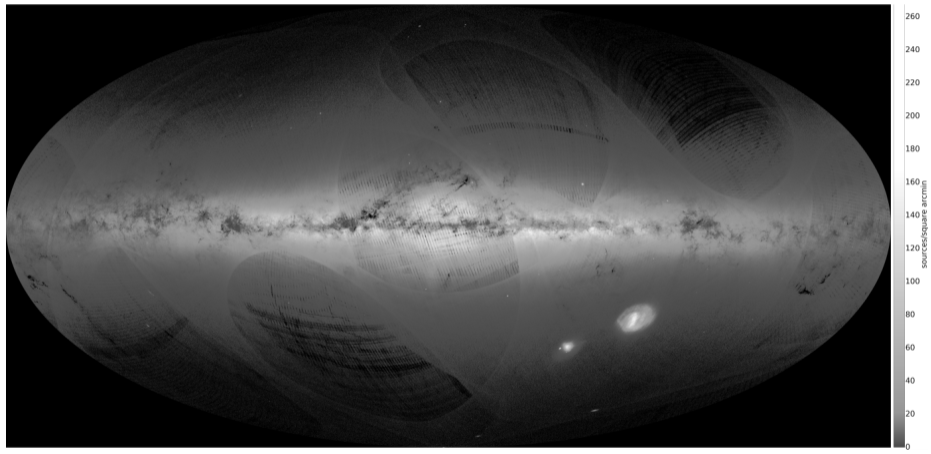
\includegraphics[width = 12cm, height = 6cm]{./Graficos/Capitulo_1/Gaia_DR1_Flux.png}} 
\caption{\scriptsize{ Sky distribution of all \textit{Gaia} DR1 sources in Galactic coordinates. The gray scale shows the source density which outlines well-known dust features along the Galactic plane in great detail. This scale also highlights non-astronomical artifacts. Image credits: CENTRA - University of Lisbon (part of the DPAC-CU9 visualization team). This figure is taken from (\cauthor{2016A&A...595A...2G} \citeyear{2016A&A...595A...2G}).}}
\label{fig:Gaia_DR1_Flux}
\end{figure}

In April $2018$ the \textit{Gaia} DR2 was released, consisting of astrometry, photometry, radial velocities, and information on astrophysical parameters and variability of sources brighter than magnitude $21.0$. In addition, epoch astrometry and photometry were provided for a modest sample of minor planets in the solar system (\cauthor{2018arXiv180409365G} \citeyear{2018arXiv180409365G}). This data release represents a major advance with respect to \textit{Gaia} DR1 in terms of completeness, performance, and richness of the data products corresponding to the first $22$ months of the mission. The data set contains celestial positions and the apparent magnitude brightness in G-band for approximately $1.7$ billion sources of which $1.3$ billion have additionally available parallaxes and proper motions \cauthor{2018arXiv180409366L} (\citeyear{2018arXiv180409366L}). There are four new key elements in this release: \textit{(i)} broad-band color information in the form of the apparent brightness in the $\textnormal{G}_\textnormal{BP}$ ($330-680\textnormal{nm}$) and $\textnormal{G}_\textnormal{RP}$ ($630-1050\textnormal{nm}$) bands, available for $1.4$ billion sources; \textit(ii) median radial velocities for some $7$ million source; \textit{(iii)} effective temperature, extinction, reddening, and radius and luminosity are provided for between $77$ and $161$ million sources; and \textit{(iv)} for a pre-selected list of $14\,000$ minor planets in the solar system epoch astrometry and photometry are provided (\cauthor{2018arXiv180409365G} \citeyear{2018arXiv180409365G}).\\ %The original sample of detections which were processed goes up to $52$ billion, but around $11$ billion were considered spurious and therefore did not take part in the cross-matching. Thus, the remaining $41$ billion transits were matched to $2\,583$ million sources, of which a significant number could be still spurious, have too few or poor observations leading to a final sample of $1693$ million sources \cauthor{2018arXiv180409366L} (\citeyear{2018arXiv180409366L}). For the bright sources ($\textnormal{G}\sim12\textnormal{mag}$), where parallax and proper motion data were already included in the \textit{Gaia} DR1, the new results represent a more accurate and fully independent of the \textit{Hipparcos} and \textit{Tycho} catalogs.\\

For \textit{Gaia} DR2 source are provided with broadband photometry in the $\textnormal{G}$,  $\textnormal{G}_\textnormal{BP}$, and  $\textnormal{G}_\textnormal{RP}$ bands (\cauthor{2017A&A...599A..32V} (\citeyear{2017A&A...599A..32V}); \cauthor{2017A&A...600A..51E} (\citeyear{2017A&A...600A..51E}); \cauthor{2018arXiv180409366L} (\citeyear{2018arXiv180409366L})). However, photometry is not perfect and strong systematic effects at the faint end of the survey $\textit{G}\sim19$, in crowded regions, and near bright stars are present. Specific treatment of crowded regions, and background estimation for the blue and red photometers lead to inconsistent measurements in different fluxes in the $\textnormal{G}$ and the $\textnormal{G}_\textnormal{BP}$, and  $\textnormal{G}_\textnormal{RP}$ bands in the sense that the sum of the flux values in the latter two bands may be significantly larger than that in $\textnormal{G}$ (whereas it is expected to be the quite same) (\cauthor{2018arXiv180409365G} \citeyear{2018arXiv180409365G}). \textit{Gaia} provides an `excess factor' entry to correct for possible photometric errors included if needed. 

%The major new element of solar information for \textit{Gaia} DR2 sources is provided by the broadband photometry in the $\textnormal{G}$,  $\textnormal{G}_\textnormal{BP}$, and  $\textnormal{G}_\textnormal{RP}$ bands (\cauthor{2017A&A...599A..32V} (\citeyear{2017A&A...599A..32V}); \cauthor{2017A&A...600A..51E} (\citeyear{2017A&A...600A..51E}); \cauthor{2018arXiv180409366L} (\citeyear{2018arXiv180409366L})). This suffers from strong systematic effects at the faint end of the survey $\textit{G}\sim19$, in crowded regions, and near bright stars. Insufficiently accurate background estimation is present in the photometric measurements from the blue and ed photometers, and from the lack of specific treatment of the prism spectra in crowded regions, where the overlapping of images of nearby sources is not yet accounted for. This basically leads to measured fluxes that are inconsistent between the $\textnormal{G}$ and the $\textnormal{G}_\textnormal{BP}$, and  $\textnormal{G}_\textnormal{RP}$ bands in the sense that the sum of the flux values in the latter two bands may be significantly larger than that in $\textnormal{G}$ (whereas it is expected that for normal spectral energy distributions the sum of fluxes in $\textnormal{G}_\textnormal{BP}$ and $\textnormal{G}_\textnormal{RP}$ should be comparable to that in $\textnormal{G}$) \cauthor{2018arXiv180409365G} (\citeyear{2018arXiv180409365G}). The \textit{Gaia} DR2 database counts with a quantitative indicator of this effect in the form of `excess factor' called \textit{phot\_bp\_rp\_excess\_factor} in the data archive in order to allow users to clean their samples and obtain reliable information.\\

In \autoref{fig:Gaia_DR2_Flux} and \autoref{fig:Gaia_DR2_FluxColor}, the sky distribution of all \textit{Gaia} DR2 sources in Galactic coordinates, and a map of the total flux measured in the $G_{RP}$, $G$, and $G_{BP}$ bands is shown. The sky map distribution shows in logarithmic scale the number of sources per square arcmin. The total flux map combines the integrated fluxes as observed in the $\textnormal{G}$,  $\textnormal{G}_\textnormal{BP}$, and  $\textnormal{G}_\textnormal{RP}$ bands, where the integrated flux map for each of the bands was used to color code the image according to a red, green, and blue channel. Here, it is evident the availability of homogeneous all-sky multi-band photometry in \textit{Gaia} DR2, offering a magnificent view of the Milky Way in color \cauthor{2018arXiv180409365G} (\citeyear{2018arXiv180409365G}). This represents the most detailed all-sky map in the optical to date. A remarkable improvement from \textit{Gaia} DR1 to \textit{Gaia} DR2 can be appreciated comparing \autoref{fig:Gaia_DR1_Flux} and \autoref{fig:Gaia_DR2_Flux} in which a much more complete and homogeneous sample is presented.\\  

\begin{figure}[!ht]
\centering
  \subfloat{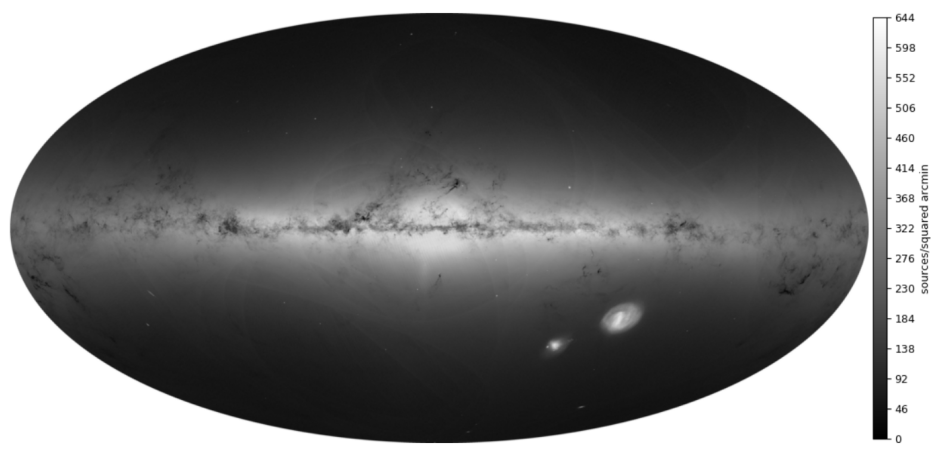
\includegraphics[width = 13cm, height = 6cm]{./Graficos/Capitulo_1/Gaia_DR2_Flux.png}} 
\caption{\scriptsize{ Sky distribution of all \textit{Gaia} DR2 sources in Galactic coordinates. This figure and the one in \autoref{fig:Gaia_DR2_FluxColor} are Hammer projections of the full sky.
The projection guarantees to have the same area per pixel (not strictly true because of pixel discretization). Each pixel is $\sim5.9$ square
arcmin. The color scale is logarithmic and represents the number of sources per square arcmin. The figure was taken from (\cauthor{2018arXiv180409365G} \citeyear{2018arXiv180409365G})}}
\label{fig:Gaia_DR2_Flux}
\end{figure}

\begin{figure}[!ht]
\centering
  \subfloat{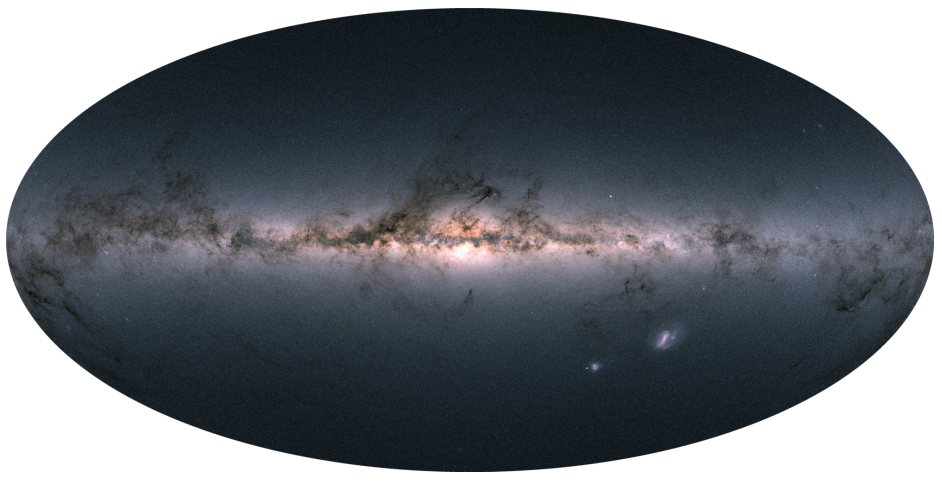
\includegraphics[width = 12.5cm, height = 6cm]{./Graficos/Capitulo_1/Gaia_DR2_FluxColor.png}} 
\caption{\scriptsize{  Map of the total flux measured in the $G_{RP}$, $G$, and $G_{BP}$ bands, where the flux in these bands is encoded in the red, green, and blue channel,
respectively. In some regions as in the lower left of the bulge there is a green region produced by lack of information in the $G_{BP}$ and $G_{RP}$ bands for a large number of sources. This kind of artifacts is also present in the region to the upper left of the Small Magellanic Cloud and at high Galactic
latitude to the right of the north Galactic pole region. The figure was taken from (\cauthor{2018arXiv180409365G} \citeyear{2018arXiv180409365G})}}
\label{fig:Gaia_DR2_FluxColor}
\end{figure}

In general, \textit{Gaia} is built to address questions on the formation and evolution of our Galaxy through the analysis of the distribution and kinematics of luminous and dark mass. By combining extinction deduced from stars, it is possible to construct the three-dimensional distribution of dust in our galaxy. In this way, \textit{Gaia} not only addresses the stellar contents, but also the interstellar matter in the Milky Way. \textit{Gaia} distances allow the derivation of absolute luminosities for stars which, combined with metallicities, allow the derivation of accurate individual ages, in particular for old subgiants, which are evolving from the main-sequence turn-off to the bottom of the red giant branch. One of the most striking and revolutionary results from this mission is the measurement of parallaxes, with hundreds of millions being accurate enough to derive high-quality color-magnitude diagrams and to make significant progress in stellar astrophysics. Star formation studies will benefit from the combination of \textit{Gaia} astrometry and photometry. On average, each star is measured astrometrically $\sim70$ times during five-year nominal operations phase. Sudden photometric changes in transient objects can be captured and the community can be alerted for follow-up observations. Periodic changes in photometry can be used to find (eclipsing) binaries and an improved census of double-lined systems based on spectroscopy will follow from the \textit{Gaia} data. A strong point of \textit{Gaia} in the exoplanet research field is the provision of an unbiased, volume-limited sample of Jupiter-mass planets in multi-year orbits around their host stars \cauthor{2014ApJ...797...14P} (\citeyear{2014ApJ...797...14P}). In addition, the astrometric data of \textit{Gaia} allow actual masses (rather than lower limits) to be measured. Besides this, the data will provide the detailed distributions of giant exoplanet properties (including the giant planet - brown dwarf transition regime) as a function of stellar-host properties with unprecedented resolution. %\textit{Gaia} will provide a census of orbital parameters and taxonomy in a single, homogeneous photometric system. A major scientific aim in the Local Group concerns the mutual, dynamical interaction of the Magellanic Clouds and the interaction between the Clouds and the Galaxy. Quasars form a special category of extragalactic sources for \textit{Gaia} as not only their intrinsic properties can be studied, but they can also be used in comparisons of optical and radio reference frames. Given the huge number of measurements, it is possible to exploit the redundancy in these corrections to conduct relativity tests or to use (residual of) the \textit{Gaia} data in more general fundamental-physics experiments.     


%==============================================================================================================================
\section{SuperWASP (Wide Angle Search for Planets)}\label{sec:SWASPdata}

Radial velocity surveys indicate that around $~1\%$ of solar neighborhood stars harbor hot Jupiter companions, and when invoking geometric arguments then $~10\%$ of these planets distributed in random orbits should transit their parent stars (\cauthor{2003ASPC..294..405S} (\citeyear{2003ASPC..294..405S}); \cauthor{2006PASP..118.1407P} (\citeyear{2006PASP..118.1407P})). Therefore, in random Galactic fields, roughly $1$ to $1000$ solar-type stars should exhibit transits lasting $\sim 2$hr with a period of a few days \cauthor{2006PASP..118.1407P} (\citeyear{2006PASP..118.1407P}). In particular, there is an apparent lack of transits due to the difficulty obtaining photometry of a sufficient number of solar-and late-type main-sequence stars. This was a strong reason back in the early 2000's to perform dense sampling to enable us to detect and closely examine the light curves of a range of transient phenomena \cauthor{2003ASPC..294..405S} (\citeyear{2003ASPC..294..405S}).\\

The \textit{SuperWASP} project is an exoplanet transit survey that has been automatically taking wide field images since $2004$. It is composed of basically two instruments (identical robotic telescopes), one located at the Observatorio del Roque de los Muchachos on La Palma, and the other one at the South African Astronomical Observatory in South Africa, continually monitoring the night sky, building up light curves of millions of unique objects (\cauthor{2006PASP..118.1407P} (\citeyear{2006PASP..118.1407P}); \cauthor{2008ApJ...675L.113W} (\citeyear{2008ApJ...675L.113W}); \cauthor{2010A&A...520L..10B} (\citeyear{2010A&A...520L..10B})). Each telescope consists of eight lenses (Canon $200$ mm f$/1.8$) feeding a $2048\times2048$ thinned CCD with a pixel size of $13.5 \mu \textnormal{m}$. This gives a field of view of $7.8\times7.8 \textnormal{deg}$ ($61\textnormal{deg}^2$) per camera \cauthor{2010A&A...520L..10B} (\citeyear{2010A&A...520L..10B}), a total field of view of $482\textnormal{deg}^2$, and an angular scale of $13.7\textnormal{px}^{-1}$ \cauthor{2006PASP..118.1407P} (\citeyear{2006PASP..118.1407P}). The delivered photometry accuracy is better than $1\%$ for objects having V$\sim7.0-11.5$. From $2006$ onwards a broadband filter was installed with a passband from $400$ to $700\textnormal{nm}$. The systems were designed to monitor fields with high cadence and they are capable of surveying the entire visible sky every $40$ minutes. The observation is carried out in $6$-$8$ fields at a similar declination and spaced apart approximately by one hour in right ascension each night. In order to avoid crowded fields close to the Galactic plane the observing strategy is altered. Thus a large part of mid-plane of the Milky Way galaxy is not sampled. Twice per night the exoplanet survey is interrupted to perform a full sky survey, a process that takes $40$ minutes as was said before \cauthor{2010A&A...520L..10B} (\citeyear{2010A&A...520L..10B}). Images are taken simultaneously from eight wide-angle cameras in each case throughout the night, offering as main product to the scientific community, light curves of individual stars \cauthor{2010A&A...520L..10B} (\citeyear{2010A&A...520L..10B})\\    

This surveys have the great advantage of requiring only relatively inexpensive, off-the-shelf equipment, which is then dedicated to the project. As said before, radial velocity surveys indicate that $\sim 1\%$ of stars between $7$ and $13$ mag may harbor hot Jupiters. Such a sample is necessary to answer questions about the formation and evolution of these planets, and how it is related to factors such as stellar metallicity, age, type, among others \cauthor{2003ASPC..294..405S} (\citeyear{2003ASPC..294..405S}). On the other hand, the main science aim of these systems is to search for bright transiting exoplanet systems suitable for spectroscopic follow-up observations \cauthor{2003ASPC..294..405S} (\citeyear{2003ASPC..294..405S}). \textit{SuperWASP} DR1 contains light curves data and images from $2$nd May $2004$ up to $9$th August $2008$ for the North hemisphere, and from $13$th February $2006$ and go through to the $27$th May $2008$ \cauthor{2010A&A...520L..10B} (\citeyear{2010A&A...520L..10B}). The data set contains in total $3\,631\,972$ raw images and $17\,970\,937$ light curves. In \autoref{fig:SWASP_DR1_Flux}, the projection of the average number of data points per light curve in the \textit{SuperWASP} DR1 is shown. Moreover, the format of the data lends itself to non-exoplanet research also, for example variable star studies \cauthor{2007A&A...467..785N} (\citeyear{2007A&A...467..785N}) and single star studies \cauthor{2007MNRAS.380.1230C} (\citeyear{2007MNRAS.380.1230C})\\  

\begin{figure}[!ht]
\centering
  \subfloat{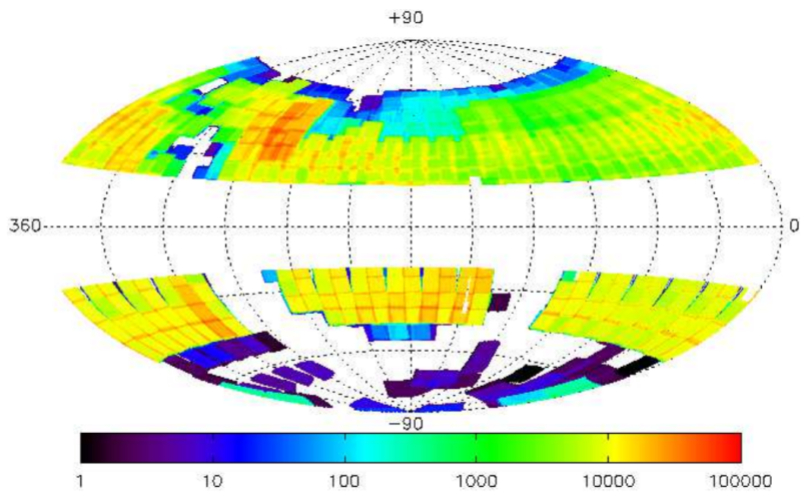
\includegraphics[width = 12cm, height = 7cm]{./Graficos/Capitulo_1/SWASP_DR1.png}} 
\caption{\scriptsize{  Hammer-Aitoff projection of the average number of data
points per light curve available in this \textit{SuperWASP} DR1. \cauthor{2010A&A...520L..10B} (\citeyear{2010A&A...520L..10B})}}
\label{fig:SWASP_DR1_Flux}
\end{figure}

\begin{table}[]
\centering
\caption{Data available for each photometric point \cauthor{2006PASP..118.1407P} (\citeyear{2006PASP..118.1407P}) in the \textit{SuperWASP} DR1 \cauthor{2010A&A...520L..10B} (\citeyear{2010A&A...520L..10B})}
\label{tab:SWASP_params}
\scalebox{0.9}{
\begin{tabular}{lll}
\hline Name          & Unit                              & Description                    \\ \hline \hline
              & Stored in the light curve on disk &                                \\ \hline
TMID          & s                                 & Mid-time of exposure           \\
FLUX2         & micro Vega                        & Processed flux                 \\
FLUX2\_ERR    & micro Vega                        & Processed flux error           \\
TAMFLUX2      & micro Vega                        & TAMUZ corrected processed flux \\
TAMFLUX2\_ERR & micro Vega                        & TAMUZ flux error               \\
CCDX          & 1/16th of pixel                   & X position on the CCD          \\
CCDY          & 1/16th of pixel                   & Y position on the CCD          \\
IMAGEID       & \_                                & Unique image ID                \\
FLAG          & \_                                & Bitmask                        \\ \hline
\end{tabular}
}
\end{table}

Each light curve is stored in binary FITS table format. In \autoref{tab:SWASP_params}, the columns in the FITS file are listed. Each row corresponds to a data point in the light curve and is the result of aperture photometry of the images by a pipeline, as described in \cauthor{2005MNRAS.364.1091K} (\citeyear{2005MNRAS.364.1091K}). This results in a processed flux measurement (\textit{FLUX2}) of each object from each image. However, further to this flux, a \textit{TAMUZ} corrected flux is given, which gives a more consistent measurement between different cameras and years (\cauthor{2007MNRAS.380.1230C} (\citeyear{2007MNRAS.380.1230C}); \cauthor{2010A&A...520L..10B} (\citeyear{2010A&A...520L..10B})). The \textit{TAMUZ} flag is a bit-mask; if corrections has been made then this will be $32$, if it is zero then the \textit{TAMUZ} flux and error will be a copy of \textit{FLUX2} values. \textit{TMID} is the heliocentrically corrected mid-point of the exposure in seconds after $2004-01-01\textnormal{T}00:00:00$ and can be converted to \textit{HJD} using \autoref{eq:HJD_Swasp}.\\ 

\begingroup
\Large
\begin{equation}
 \textnormal{HJD} = \frac{\textnormal{TMID}}{86\,400} + 2453005.5 
 \label{eq:HJD_Swasp}
\end{equation}
\endgroup

\begingroup
\Large
\begin{equation}
 \textnormal{mag} = 15.0 - 2.5 \log(\textnormal{flux})
 \label{eq:Mag_Swasp}
\end{equation}
\endgroup \\

In both flux cases the units are given as micro Vegas, this gives a simple conversion given by \autoref{eq:Mag_Swasp}, where flux is in micro Vegas. This implies a flux of $1.0$ micro Vega corresponds to $15$th mag, and $10^6$ micro Vega; $0th$ mag \cauthor{2010A&A...520L..10B} (\citeyear{2010A&A...520L..10B}). Last but not least, the names of each star in the \textit{SuperWASP} are listed as follows, $1\textnormal{SWASP}~~\textnormal{Jhhmmss.ssSddmmss.s}$. Therefore, following this convention, a unique identifier is used. 

%==============================================================================================================================
\section{Sco OB2 (ScoCen)}\label{sec:ScoOB2}

This project was centered in a region of the night sky known as Sco OB2 or ScoCen. The region was classified as an OB association by \cauthor{Blaauw46} (\citeyear{Blaauw46}) due to the fact that back in the days only more massive stars were achievable through photometric studies mainly made up of O/B-type stars. However, nowadays is quite clear that OB associations contain members across the mass spectrum, including not only O-and B-type stars, but also intermediate mass A/F stars, lower-mass G/K/M stars, and very low-mass free floating substellar objects. Stars below $< 1.5 \textnormal{M}_\odot$ comprise the dominant component of OB associations which is equivalent to say that the vast majority correspond to low-mass stars \cauthor{2016MNRAS.461..794P} (\citeyear{2016MNRAS.461..794P}).\\

ScoCen is the nearest OB association to the Sun that has recently formed stars \cauthor{2018MNRAS.tmp..210W} (\citeyear{2018MNRAS.tmp..210W}), turning it into one of the most important OB associations to study the star-formation process, the origin of the initial mass function (IMF), to investigate how high-and low-mass stars are distributed in space during the evolution of the giant molecular clouds and the star-forming process \cauthor{1989A&A...216...44D} (\citeyear{1989A&A...216...44D}) and the interaction of early-type stars with the interstellar medium. In particular, these regions offer an indispensable good sample to characterize and study the formation of planets and their evolution allowing us to estimate the timescale in which gaseous disks dissipate \cauthor{2018arXiv180200878M} (\citeyear{2018arXiv180200878M}), and the potential of a star to host habitable exoplanets which is directly related to the environment on which stars are born and spend the first few million years of their lives \cauthor{2018MNRAS.tmp..210W} (\citeyear{2018MNRAS.tmp..210W}). Also indispensable for direct imaging of brown dwarf and planetary mass companions; star disk interaction of young stars, imaging of debris disks, and evolution of gas-rich and dusty debris disks \cauthor{2016MNRAS.461..794P} (\citeyear{2016MNRAS.461..794P}). It is widely known that stars tend to form in clusters, however, stars with ages around $\sim10 \textnormal{Myr}$ observed in bound clusters only account for a $10\%$ in total. A likely explanation to this is based on how stars are formed embedded within molecular clouds, which are indeed held together by their own gravitational potential of both stars and gas \cauthor{2018MNRAS.tmp..210W} (\citeyear{2018MNRAS.tmp..210W}), but when the intern feedback disperses the gas, then the cluster starts to disperse and expand. This is why we can observe low-density groups of young stars known as associations that can keep on evolving and disperse in the galactic field.\\

Since its discovery, the region has been divided in three main subgroups known as \textit{Upper Scorpius} (US), \textit{Upper Centaurus-Lupus} (US), and \textit{Lower Centaurus-Crux} (LCC) \cauthor{Blaauw46} (\citeyear{Blaauw46}), with mean parallaxes of $6.9$, $7.1$, and $8.5$mas or distances of $145$, $143$, and $118$pc respectively \cauthor{2015yCat..74163108R} (\citeyear{2015yCat..74163108R}). In recent studies as those of \cauthor{2018MNRAS.tmp..210W} (\citeyear{2018MNRAS.tmp..210W}) this OB association has been proposed to lie in a distance range between $\sim100$ to $150$ pc covering almost $90$-deg on the sky or $2000\textnormal{deg}^2$. The estimated ages of US, UCL, and LCC are $11$, $16$, and $17$ Myr respectively, though it is clear that there exists a considerable spread (\cauthor{1989A&A...216...44D} \citeyear{1989A&A...216...44D}; \cauthor{2018MNRAS.tmp..210W} \citeyear{2018MNRAS.tmp..210W}). US contains a vast number of stars that has been thoroughly studied in the past decades, however, it is clear the LCC and UCL are more spread out decreasing the concentration and making the task more tricky due to the closer overlap with the Galactic plane \cauthor{2015yCat..74163108R} (\citeyear{2015yCat..74163108R}) making the separation of actual member really difficult. High quality data is needed, as measurements of star motions which allows the study of the separation of UCL and LCC members as provided by surveys as \textit{Hipparcos} \cauthor{1999AJ....117..354D} (\citeyear{1999AJ....117..354D}) and \textit{Gaia} DR1-DR2 (\cauthor{2012yCat..74163108R} \citeyear{2012yCat..74163108R}; \cauthor{2016MNRAS.461..794P} \citeyear{2016MNRAS.461..794P}; \cauthor{2018MNRAS.tmp..210W} \citeyear{2018MNRAS.tmp..210W}). \textit{Gaia} DR2 provides provides a remarkable improvement in parallaxes and proper motions of stars for the ScoCen region that for example benefits studies of the dynamical situation of the cluster to prove expansion, and constraint the initial conditions as those performed by \cauthor{2018MNRAS.tmp..210W} (\citeyear{2018MNRAS.tmp..210W}). In \autoref{fig:ScoCen_Mamajek}, a current sample of $433$ ScoCen members was used by \cauthor{2018MNRAS.tmp..210W} (\citeyear{2018MNRAS.tmp..210W}) to add additional information to the known properties of the OB association cross-matching \textit{Gaia} DR1 parallaxes and proper motion for a few of these sources.\\   

\begin{figure}[!ht]
\centering
  \subfloat{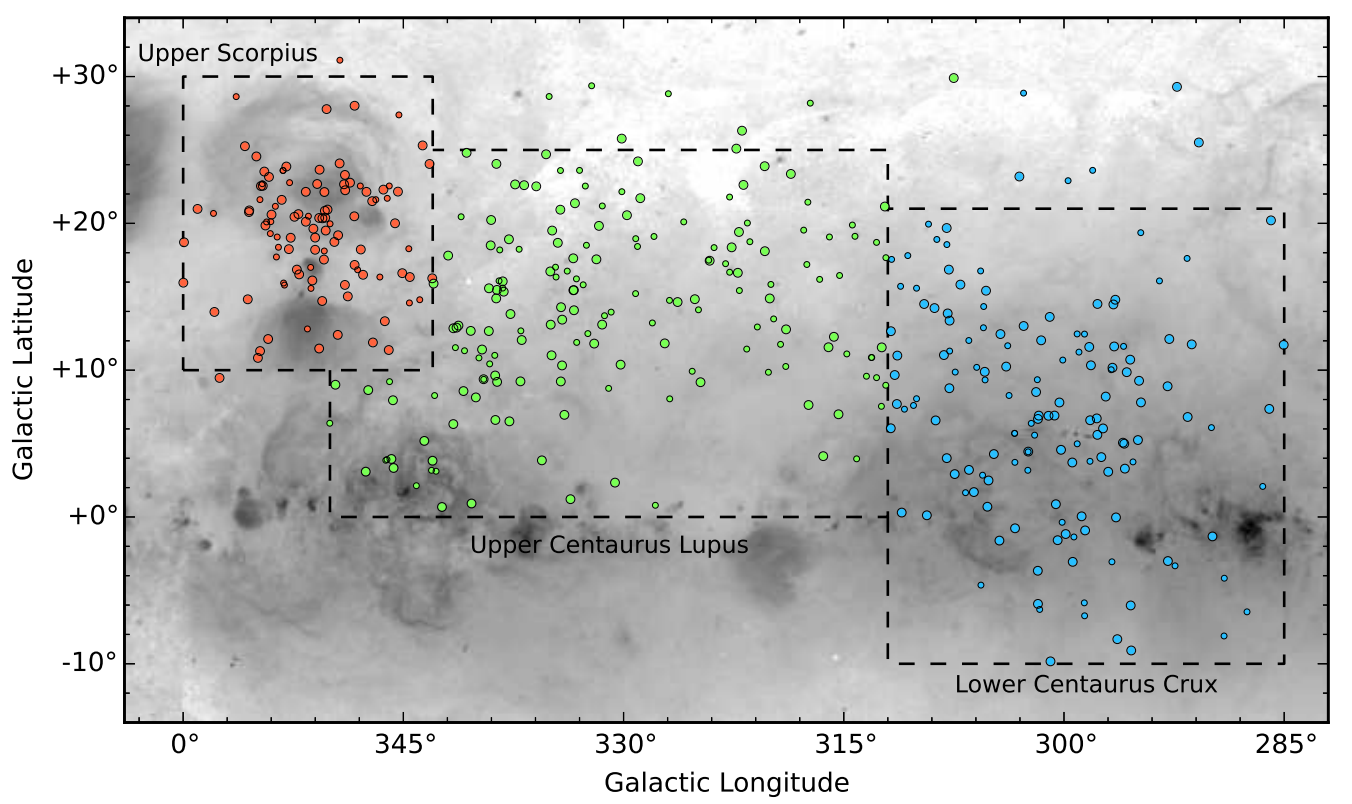
\includegraphics[width = 15cm, height = 8.5cm]{./Graficos/Capitulo_1/ScoCen.png}} 
\caption{\scriptsize{ Sco OB2 association in galactic coordinates. The dashed-line squares represent from top to bottom the Upper Scorpius, Upper Centaurus-Lupus, and Lower Centaurus-Crux regions as defined by \cauthor{Blaauw46} (\citeyear{Blaauw46}) and redefined by \cauthor{1999AJ....117..354D} (\citeyear{1999AJ....117..354D}). The sample corresponds to a total number of $433$ stars colored according to which of the three subgroups they nominally belong to. This figure is taken from \cauthor{2018MNRAS.tmp..210W} (\citeyear{2018MNRAS.tmp..210W}).}}
\label{fig:ScoCen_Mamajek}
\end{figure}

In \autoref{fig:ScoCen_Mamajek} a modified version of the original boundaries \cauthor{Blaauw46} (\citeyear{Blaauw46}) for the subgroups as re-defined by \cauthor{1999AJ....117..354D} (\citeyear{1999AJ....117..354D}) is presented. In general, the US, UCL, and LCC subgroups have been limited in total proper motion to $\mu < 47$, $12 < \mu < 55$, and $15 < \mu < 55$ mas respectively, and $\mu^*_\alpha < 10$ and $\mu_\delta < 30$ mas for the three subgroups \cauthor{2016MNRAS.461..794P} (\citeyear{2016MNRAS.461..794P}). Additionally, the low-mass population in ScoCen has been studied before focusing on binary properties, circumstellar disks, stellar ages, eclipsing binaries, and low-mass stars and brown dwarfs. This is particularly useful to study the early evolution of low-mass stars and substellar objects which requires an excellent characterization of young low-mass objects \cauthor{2018arXiv180200878M} (\citeyear{2018arXiv180200878M}) to give a glimpse into the state of a group of stars directly after their formation, and using a unique age-calibrated sample \cauthor{2015yCat..74163108R} (\citeyear{2015yCat..74163108R}).  

%==============================================================================================================================
\section{Exoplanetary Rings: the particular case of J1407}\label{sec:Exorings}

% Mamamjek 2012  \cauthor{2012AJ....143...72M} (\citeyear{2012AJ....143...72M}
% Kenworthy 2015 \cauthor{2015MNRAS.446..411K} (\citeyear{2015MNRAS.446..411K}
% \cauthor{} (\citeyear{}

Exoplanetary transits have been a major topic in astrophysics since the 1990's when the first exoplanets were discovered. The vast sample was mainly conformed by giant planets and Hot-Jupiters. Since then, different techniques as radial velocity, transit photometry, direct imaging, among others have been explored and refined to achieve lower limits which allows us to detect earth-like planets. However, less is said about circumplanetary disks (proto-satellite disks) that likely existed during the first $\sim10^7$ years \cauthor{2012AJ....143...72M} (\citeyear{2012AJ....143...72M}), although, there are studies investigating the detectability of thin, discrete planetary rings similar to Saturn's as reported in (\cauthor{2004ApJ...616.1193B} \citeyear{2004ApJ...616.1193B}; \cauthor{2009ApJ...690....1O} \citeyear{2009ApJ...690....1O}). Circumplanetary disks are extended, then, the probability that a randomly oriented system exhibits eclipses may not be negligible. In \cauthor{2012AJ....143...72M} (\citeyear{2012AJ....143...72M}), it was estimated that a survey of $\sim10^4$ young ($~10$ million year old) post-accretion pre-main-sequence stars monitored for $~10$ years should yield at least a few deep eclipses from circumplanetary disks and disks surrounding low-mass companion stars.\\
 
In $2012$, \cauthor{2012AJ....143...72M} (\citeyear{2012AJ....143...72M}) identified a star with a remarkable light curve among the \textit{SuperWASP} DR1 data (\cauthor{2006PASP..118.1407P} \citeyear{2006PASP..118.1407P}; \cauthor{2010A&A...520L..10B} \citeyear{2010A&A...520L..10B}) for the new ScoCen members known as \textit{1SWASP J1407.93-394542.6 = ASAS J140748-3945.7} (hereafter `J1407'). This star is known to be part of the \textit{Upper Centaurus-Lupus} subgroup of ScoCen \cauthor{1999AJ....117..354D} (\citeyear{1999AJ....117..354D}) lying at a distance of $128\pm13$ pc derived from a kinematic analysis, similar to the UCL members as reported by \cauthor{2012AJ....143...72M} (\citeyear{2012AJ....143...72M}). Using this distance, and three sets of evolutionary tracks, the star is known to be located in the HR-diagram at $\log$ T $= 3.66$ and $\log$ L$/$L $=$ -0.47 with a stellar mass of $\sim0.9$M$_\odot$. The young star ($\sim 16$ Myr) appears to be a weak-lined T Tauri star, not hosting its own circumstellar disk \cauthor{2015MNRAS.446..411K} (\citeyear{2015MNRAS.446..411K}). \\ 

In particular, the light curve exhibited a notorious long, deep, and complex eclipse event centered on $2007$ April $29$th as seen in the \textit{SuperWASP} V-magnitude photometry, and with portions of the dimming confirmed by the All Sky Automated Survey (\textit{ASAS}) \cauthor{2002AcA....52..397P} (\citeyear{2002AcA....52..397P}) data as it is shown in \autoref{fig:Mamajek_J1407_1}. This unusual eclipse is similar to those seen in $\epsilon$ Aurigae (\cauthor{2002ASPC..279..121G} \citeyear{2002ASPC..279..121G}; \cauthor{2010Natur.464..870K} \citeyear{2010Natur.464..870K}; \cauthor{2011A&A...530A.146C} \citeyear{2011A&A...530A.146C}), KH 15D \cauthor{2006ApJ...644..510W} (\citeyear{2006ApJ...644..510W}), EE Cep (\cauthor{Mikolajewski1999} \citeyear{Mikolajewski1999}; \cauthor{2003A&A...403.1089G} \citeyear{2003A&A...403.1089G}; \cauthor{2010ASPC..435..423G} \citeyear{2010ASPC..435..423G}) which are periodically occulted by extended objects. The \textit{SuperWASP} DR1 photometry contains approximately $29\,000$ epochs during $206$ dates between HJD $2453860$ ($2006.34$) and HJD $2455399$ ($2010.56$), with median photometric precision  of $0.023$ mag. On the other hand, the \textit{ASAS} archive contains an extremely long time baseline light curve for J1407, with photometry provided over 599 dates between HJD $2451887$ $2001$ February and HJD $2455088$ $2009$ September. In this dataset sample, a minor but sustained dip in magnitudes between $2001.20$ and $2001.24$, approximately $14$ days and with depth $\sim 0.2$ mag is also observed.\\

Five multi-day dimming events of $>0.5$ mag were identified, with a $3.3$ mag deep eclipse between HJD $2454213$ ($2007$ April $23$rd) and HJD $ 2454227$ ($2007$ May $7$th), bracketed by two pairs of $\sim 1$ mag eclipses symmetrically occurring $\pm 12$ days and $\pm 26$ days before and after, as reported in \cauthor{2012AJ....143...72M} (\citeyear{2012AJ....143...72M}). The light curve for the \textit{SuperWASP} data is dominated by a quasi-sinusoidal component with amplitude $\sim0.1$ mag and periodicity of $3.211$ days consistent with rotational modulation of starspots, typical for young active stars \cauthor{2008ApJ...687.1264M} (\citeyear{2008ApJ...687.1264M}). A firm lower limit on the period of $850$ days was placed by \cauthor{2012AJ....143...72M} (\citeyear{2012AJ....143...72M}). In right panel of \autoref{fig:Mamajek_J1407_1}, both data from nightly averaged \textit{SWASP}, and \textit{ASAS} is shown, where two pairs of multiday dips named $A1$ and $A2$ separated by $\sim24$ days, and $B1$ and $B2$ separated by $\sim51.5$ days can be observed. From this figure, it is inferred that probably a disk with large gaps may be producing extra dips in between those pairs mentioned above, because they appear to be free of extinction lasting just for a couple of days.\\      
 
\begin{figure}[!ht]
\centering
  \subfloat{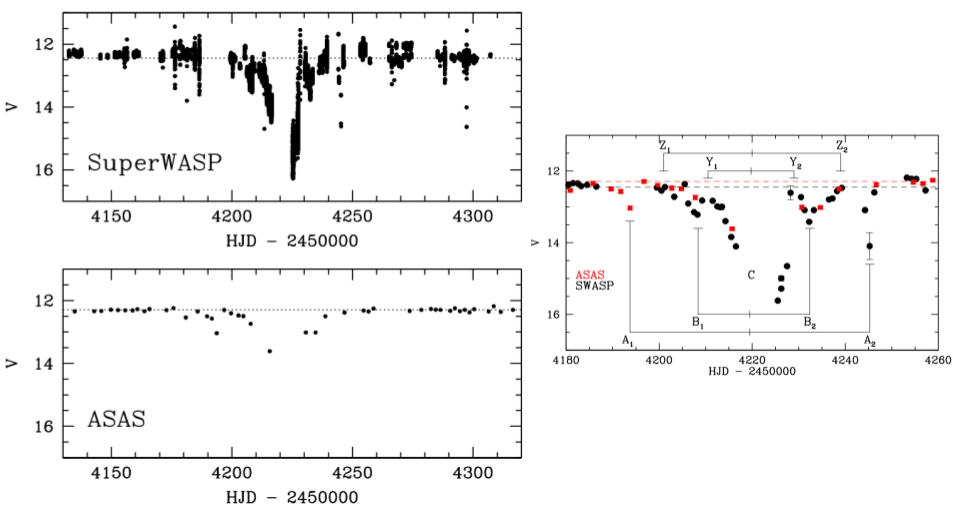
\includegraphics[width = 16cm, height = 10cm]{./Graficos/Capitulo_1/Mamajek_J1407.png}} 
\caption{\scriptsize{ \textbf{Top left:} \textit{SuperWASP} V-magnitude light curve for J1407. \textbf{Bottom left:} \textit{ASAS} V-magnitude data for J1407 . The data was obtained during early $2007$. The abscissa corresponds to the Heliocentric Julian Date minus $2450000$. Thus, $2007$ January $1$st midnight corresponds to HJD $2454101.5$. The eclipse was seen in both photometric data sets. \textbf{right:} \textit{SuperWASP} and \textit{ASAS} photometry for the $2007$ April-May eclipse event(s). \textit{ASAS} photometry is a single measurement each night, whereas the \textit{SuperWASP} magnitudes are nightly median values. The figures are taken from \cauthor{2012AJ....143...72M}(\citeyear{2012AJ....143...72M})}}
\label{fig:Mamajek_J1407_1}
\end{figure}

Having said that, it is quite likely that the observed features  in the light curve of J1407 are being produced by a low-mass object hosting a disk with significant substructure composed of thin dust debris belts, or rings as it is shown in \autoref{fig:Mamajek_J1407} where a non-unique disk model was fit to the \textit{SuperWASP} observations. Nevertheless, a low mass secondary star with a disk, a brown dwarf, and a gas giant planet could perhaps be some plausible explanations of the features observed. This young, Li-rich K5 star, shows a lack of infrared excess emission at long (\textit{WISE}, \cauthor{2010AJ....140.1868W} (\citeyear{2010AJ....140.1868W}) and short wavelengths (\textit{WISE}, \cauthor{2006AJ....131.1163S} (\citeyear{2006AJ....131.1163S})  and no accretion indicators \cauthor{2012AJ....143...72M}(\citeyear{2012AJ....143...72M}) which clearly suggests that the mass of the unseen object is much lower than that of the solar-mass K star. On the other hand, as was stated before, the disk must be large, so the probability of a system hosting one which is oriented in such a way that can occult the star and produce the transit is tiny, but not zero. The lifetime of a second phase Jupiter's circumstellar disk is estimated to be of order a million years (\cauthor{2009euro.book...59C} (\citeyear{2009euro.book...59C}); \cauthor{2005A&A...434..343A} (\citeyear{2005A&A...434..343A}); \cauthor{2010AJ....140.1168W} (\citeyear{2010AJ....140.1168W}), thus, the lifetime of a circumplanetary disk at $25$ AU could be about $10$ times longer (or of order $\sim10^7$ years) or at $100$ AU $100$ times longer (or of order $\sim10^8$ years) \cauthor{2012AJ....143...72M} (\citeyear{2012AJ....143...72M}). Having said that, it is clear that the lifetime of a circumplanetary disk could be longer for planets at large semi-major axis, then light detected from outer exoplanets may also come from such a disk. According to \cauthor{2015MNRAS.446..411K} (\citeyear{2015MNRAS.446..411K}), the complex ring system appears to occupy more than $0.15$ of its Hill radius, much larger than its Roche radius, suggesting a ring structure in transition.\\

\begin{figure}[!ht]
\centering
  \subfloat{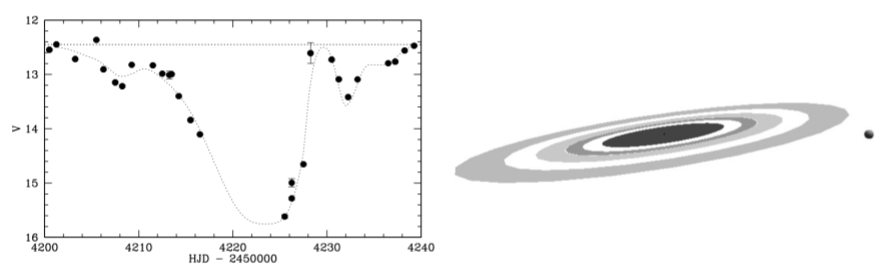
\includegraphics[width = 15cm, height = 5cm]{./Graficos/Capitulo_1/Rings.png}} 
\caption{\scriptsize{ \textbf{left:} Simple, non-unique model in an attempt to fit the nightly averaged data obtained by the \textit{SuperWASP} observations. The model contains an object orbiting J1407 composed by a thick inner disk, a gap, and two rings with a smaller gap between them. \textbf{right:} Diagram of J1407's dust disk model, whose corresponding light curve is shown in the left panel. The dark dot corresponds to J1407 to scale (R = $0.96$R$_\odot$). The figures are taken from \cauthor{2012AJ....143...72M}(\citeyear{2012AJ....143...72M})}}
\label{fig:Mamajek_J1407}
\end{figure}

Summing up, this kind of eclipses seen among young stars may provide useful constraints on either circumsecondary or circumplanetary disk structure and the early evolution of planets and/or satellites because they constitute remarkable laboratories for testing these scenarios. Same can be said in the case of J1407, regardless of the nature of the disked companion. Predicting when the next eclipse will happen is vital to planning an extensive and detailed observing campaign, and also because this object offers the opportunity to analyze a young substellar object and possibly resolve the disk with ring-like structure spectrally and spatially \cauthor{2015MNRAS.446..411K} (\citeyear{2015MNRAS.446..411K}). Additional constraints based on high spectral resolution and precision RV measurements, combined with orbital periods ruled out by photometric monitoring and dynamical arguments show that the companion of J1407 is a substellar object and likely to be a planetary mass or brown dwarf mass object. The ring system is also considerably larger than the Roche radius for the secondary companion, suggesting that the system may be in a transitional state where exomoons are in process of formation. All models imply a ring system for J1407 that fills at least $0.15$ of the Hill sphere and is significantly larger than the Roche radius \cauthor{2015MNRAS.446..411K} (\citeyear{2015MNRAS.446..411K}). These large rings are unstable on long-timescales and will ultimately accrete to form exomoons, contrasting with solar system models where moons are formed from gradual overflow over the Roche radius \cauthor{2012Sci...338.1196C} (\citeyear{2012Sci...338.1196C}).   